% Provenance (never printed): see sources/outline_sources.md (Year 2: Goldschmidt's
% classification; the chondritic Earth; core, mantle and crust compositions; trace
% elements and normalised diagrams). Curves from figdata/bachelor-2/geochem.py; exercise
% and problem values in the Book 4 scratch calculator calc/ch03.py.
\chapter{Los elementos en la Tierra}\label{ch:b2:elements-in-the-earth}

Una tonelada de las rocas de los continentes contiene alrededor de un miligramo y medio de
oro. Una tonelada de las \omterm{def:b2:planet-formation-meteorites:chondrule}{condritas carbonáceas} del capítulo anterior, las piedras más
primitivas que caen del cielo, contiene unas cien veces más. La
Tierra se ensambló con un material así, de modo que el oro no falta en la
Tierra: está en otra parte. Si se combinan las composiciones estimadas del núcleo y de
la Tierra silicatada con la masa del núcleo, resulta que más del 99 por ciento del
oro de la Tierra está en el núcleo, adonde se hundió con el hierro al principio de
la historia terrestre. El oro pertenece a una familia de elementos que siguen al hierro
metálico; otros siguen al sulfuro, otros a la roca silicatada, y otros escapan
al aire. Este capítulo clasifica los elementos en estas familias, usa las
\omterm{def:b2:planet-formation-meteorites:chondrule}{condritas} para reconstruir la composición de la Tierra entera y para pesar su
núcleo, describe las composiciones del manto, de la corteza oceánica y de la
corteza continental, e introduce los \omterm{def:b2:elements-in-the-earth:trace}{elementos en trazas} y los diagramas en los que
los geoquímicos leen la historia de una roca.
% ledger: rg03:ucc-trace, lodders:ci-table, mcd03:core, ms95:pm-trace, data:prem

\begin{recall}
La Tierra tiene un núcleo metálico, sobre todo de hierro, bajo un manto de silicatos y una delgada
corteza; la sismología da el radio y la densidad de cada capa, y el núcleo
es entre un 5 y un 10 por ciento menos denso de lo que sería el hierro puro a la misma presión y
temperatura, lo que exige elementos ligeros en él: el silicio, el azufre, el carbono,
el oxígeno y el hidrógeno son los candidatos (volumen de primer año). La
electronegatividad de un elemento mide la fuerza con que sus átomos atraen los
electrones de un enlace, y el radio de un ion depende de su carga y del
número de sus vecinos (volumen de primer año de los libros de química). Un coeficiente
de reparto es el cociente de las concentraciones de una sustancia en dos fases en
equilibrio (volumen de primer año de los libros de química). Las \omterm{def:b2:planet-formation-meteorites:chondrule}{condritas}, las \omterm{def:b2:planet-formation-meteorites:chondrule}{condritas
carbonáceas} y la \omterm{def:b2:planet-formation-meteorites:condensation}{secuencia de condensación} se presentaron en el
\cref{ch:b2:planet-formation-meteorites}.
\end{recall}
% ledger: badro:core

\section{La clasificación de Goldschmidt}

Cuando un cuerpo condrítico se funde, su materia se separa en líquidos inmiscibles: un
metal denso de hierro y níquel, un líquido sulfurado si hay suficiente azufre, y un
fundido silicatado, con una fase gaseosa por encima. Cada elemento se reparte entre
estas fases según su química, y el mismo reparto se observa en la
metalurgia, donde el hierro fundido, una mata de sulfuros y una escoria silicatada se separan en el
horno.

\begin{definition}[Clasificación de Goldschmidt]
\label{def:b2:elements-in-the-earth:goldschmidt}
La \emph{clasificación de Goldschmidt}\index{clasificación de Goldschmidt} ordena
los elementos según la fase que prefieren en un cuerpo que se separa en metal,
sulfuro, silicato y gas. Un \emph{elemento litófilo}\index{elemento litófilo}
prefiere el silicato y el óxido; un \emph{elemento siderófilo}\index{elemento siderófilo}
prefiere el hierro metálico; un \emph{elemento
calcófilo}\index{elemento calcófilo} prefiere el sulfuro; un \emph{elemento
atmófilo}\index{elemento atmófilo} permanece en el gas, como gas o como compuesto
volátil.
\end{definition}

Las clases siguen la química del enlace. Los \omterm{def:b2:elements-in-the-earth:goldschmidt}{elementos litófilos}, como los metales
alcalinos y alcalinotérreos, el aluminio, el titanio o las \omterm{def:b2:elements-in-the-earth:ree}{tierras raras}, ceden
fácilmente sus electrones al oxígeno, mucho más electronegativo, y
forman con él enlaces iónicos. Los \omterm{def:b2:elements-in-the-earth:goldschmidt}{elementos siderófilos}, los metales del grupo del platino, el oro,
el níquel y el cobalto, tienen electronegatividades cercanas a la del hierro, se enlazan débilmente
con el oxígeno y se disuelven en el metal. Los \omterm{def:b2:elements-in-the-earth:goldschmidt}{elementos calcófilos}, entre ellos el cobre, el cinc, el plomo,
la plata y el cadmio, forman con el azufre enlaces más covalentes.
Los \omterm{def:b2:elements-in-the-earth:goldschmidt}{elementos atmófilos} son los gases nobles, el nitrógeno y el hidrógeno. Muchos
elementos pertenecen a dos clases, según las condiciones: el propio hierro es
siderófilo en un cuerpo rico en metal y litófilo en el manto oxidado, donde
está en el olivino y el piroxeno; el wolframio y el molibdeno son siderófilos en la
Tierra, pero buena parte de ellos se quedó en el manto (figura siguiente).

\begin{omfigure}
\centering
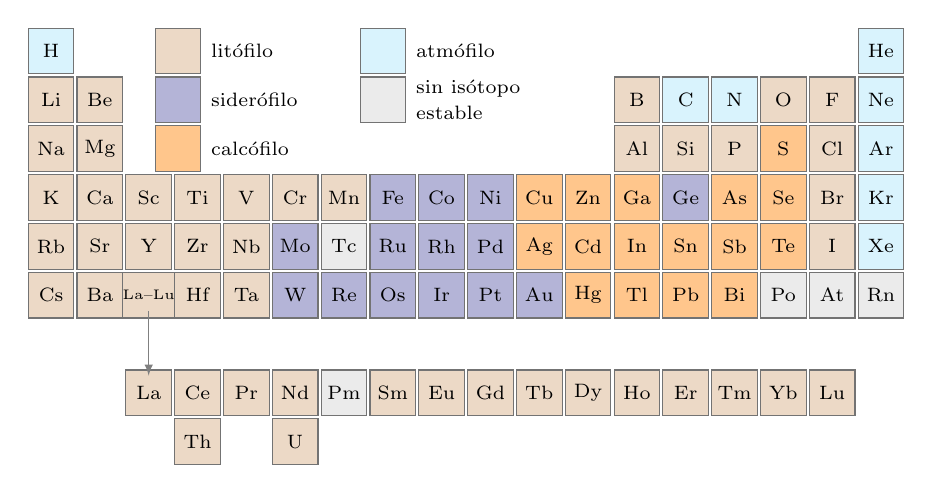
\begin{tikzpicture}[x=0.62cm, y=-0.62cm,
  lith/.style={fill=brown!30}, sid/.style={fill=blue!30!gray!45},
  chal/.style={fill=orange!45}, atm/.style={fill=cyan!15}, none/.style={fill=black!8},
  cell/.style={draw=black!55, minimum size=0.58cm, inner sep=0pt, font=\scriptsize}]
\foreach \s/\c/\r/\k in {H/1/1/atm, He/18/1/atm,
  Li/1/2/lith, Be/2/2/lith, B/13/2/lith, C/14/2/atm, N/15/2/atm, O/16/2/lith,
  F/17/2/lith, Ne/18/2/atm,
  Na/1/3/lith, Mg/2/3/lith, Al/13/3/lith, Si/14/3/lith, P/15/3/lith, S/16/3/chal,
  Cl/17/3/lith, Ar/18/3/atm,
  K/1/4/lith, Ca/2/4/lith, Sc/3/4/lith, Ti/4/4/lith, V/5/4/lith, Cr/6/4/lith,
  Mn/7/4/lith, Fe/8/4/sid, Co/9/4/sid, Ni/10/4/sid, Cu/11/4/chal, Zn/12/4/chal,
  Ga/13/4/chal, Ge/14/4/sid, As/15/4/chal, Se/16/4/chal, Br/17/4/lith, Kr/18/4/atm,
  Rb/1/5/lith, Sr/2/5/lith, Y/3/5/lith, Zr/4/5/lith, Nb/5/5/lith, Mo/6/5/sid,
  Tc/7/5/none, Ru/8/5/sid, Rh/9/5/sid, Pd/10/5/sid, Ag/11/5/chal, Cd/12/5/chal,
  In/13/5/chal, Sn/14/5/chal, Sb/15/5/chal, Te/16/5/chal, I/17/5/lith, Xe/18/5/atm,
  Cs/1/6/lith, Ba/2/6/lith, Hf/4/6/lith, Ta/5/6/lith, W/6/6/sid, Re/7/6/sid,
  Os/8/6/sid, Ir/9/6/sid, Pt/10/6/sid, Au/11/6/sid, Hg/12/6/chal, Tl/13/6/chal,
  Pb/14/6/chal, Bi/15/6/chal, Po/16/6/none, At/17/6/none, Rn/18/6/none,
  La/3/8/lith, Ce/4/8/lith, Pr/5/8/lith, Nd/6/8/lith, Pm/7/8/none, Sm/8/8/lith,
  Eu/9/8/lith, Gd/10/8/lith, Tb/11/8/lith, Dy/12/8/lith, Ho/13/8/lith,
  Er/14/8/lith, Tm/15/8/lith, Yb/16/8/lith, Lu/17/8/lith,
  Th/4/9/lith, U/6/9/lith}
  \node[cell, \k] at (\c,\r) {\s};
\node[cell, lith, minimum width=0.58cm] at (3,6) {\tiny La--Lu};
\draw[black!50, -latex] (3,6.32) -- (3,7.65);
% legend
\foreach \k/\t/\x/\y in {lith/litófilo/3.6/1, sid/siderófilo/3.6/2,
  chal/calcófilo/3.6/3, atm/atmófilo/7.8/1, none/{\shortstack[l]{sin isótopo\\estable}}/7.8/2}
  \node[cell, \k, label={[font=\scriptsize]east:\t}] at (\x,\y) {};
\end{tikzpicture}
\par\smallskip{\small Las clases de Goldschmidt de los elementos estables y del torio y el uranio, cuyos isótopos de vida larga sobreviven desde el nacimiento de la Tierra, coloreadas según la clase
que domina en la Tierra; los elementos de la fila de las \omterm{def:b2:elements-in-the-earth:ree}{tierras raras} están en la casilla
La--Lu. Varios elementos pertenecen a dos clases: el hierro, el níquel y el cobalto son también
litófilos en el manto oxidado; el carbono es también siderófilo, y el fósforo
siderófilo en los \omterm{def:b2:planet-formation-meteorites:fall-find}{meteoritos}.}
\end{omfigure}

\section{La Tierra condrítica}

Nadie puede muestrear la Tierra en su conjunto: el núcleo está fuera de alcance, y el
manto solo llega a la superficie en fragmentos. La composición de la Tierra global
se construye en cambio a partir de dos tipos de datos: los \omterm{def:b2:planet-formation-meteorites:fall-find}{meteoritos}, que muestrean el
material a partir del cual se formaron los planetas, y las rocas del manto y los
fundidos que proceden de él.

\begin{definition}[Condrita CI]\label{def:b2:elements-in-the-earth:ci}
Una \emph{condrita CI}\index{condrita CI} es un miembro del grupo de
\omterm{def:b2:planet-formation-meteorites:chondrule}{condritas carbonáceas} que lleva el nombre del \omterm{def:b2:planet-formation-meteorites:fall-find}{meteorito} de Ivuna: piedras negras y deleznables
formadas casi por completo por matriz de grano fino, ricas en minerales hidratados y en
carbono, casi sin \omterm{def:b2:planet-formation-meteorites:chondrule}{cóndrulos}. Aparte del hidrógeno, el carbono, el nitrógeno, el oxígeno y los
gases nobles, su composición es la más cercana, de todos los materiales conocidos, a la de
la fotosfera del Sol; son la composición de referencia de la geoquímica.
\end{definition}

El grupo cuenta con cinco \omterm{def:b2:planet-formation-meteorites:fall-find}{meteoritos}, todos ellos caídas: Alais (1806), Orgueil
(1864), Tonk (1911), Ivuna (1938) y Revelstoke (1965); Orgueil es el mayor,
con catorce kilogramos. La composición adoptada para el grupo es una media ponderada
de sus análisis, elemento por elemento; los valores usados en este capítulo se
citan donde hacen falta.
% ledger: lodders:ci-table

\begin{definition}[Elementos refractarios y volátiles]
\label{def:b2:elements-in-the-earth:volatility}
Un \emph{elemento refractario}\index{elemento refractario} es aquel cuya \omterm{def:b2:planet-formation-meteorites:condensation}{temperatura de condensación}
al 50 por ciento (\cref{ch:b2:planet-formation-meteorites}) es superior a
las del magnesio, el silicio y el hierro, \qtyrange{1310}{1340}{K} a
\qty{e-4}{bar}; un
\emph{elemento volátil}\index{elemento volátil} es aquel cuya \omterm{def:b2:planet-formation-meteorites:condensation}{temperatura de condensación}
es inferior a ellas.
\end{definition}

El contenido en magnesio sirve de patrón. El magnesio es litófilo, condensa
con el grueso de la roca y no entra en el núcleo, de modo que la razón de un elemento
al magnesio en la Tierra silicatada, dividida por la misma razón en las \omterm{def:b2:elements-in-the-earth:ci}{condritas CI},
mide cuánto de ese elemento conservó la Tierra silicatada respecto a un
material de partida condrítico. El agua, el carbono y los demás compuestos volátiles que
contienen las \omterm{def:b2:elements-in-the-earth:ci}{condritas CI}, y que la Tierra no conservó, se eliminan de la razón.

\begin{definition}[Tierra silicatada global, manto primitivo]
\label{def:b2:elements-in-the-earth:bse}
La \emph{Tierra silicatada global}\index{Tierra silicatada global} es la Tierra sin
su núcleo: el manto, la corteza, el océano y la atmósfera tomados juntos, como estarían si se
mezclaran. La misma composición se llama \emph{manto primitivo}\index{manto primitivo}:
el manto tal como era después de formarse el núcleo y antes de que se extrajera de él
ninguna corteza.
\end{definition}

Las estimaciones del \omterm{def:b2:elements-in-the-earth:bse}{manto primitivo} se basan en las rocas del manto que han perdido
menos fundido, peridotitas subidas como xenolitos en lavas (fotografía siguiente) o
expuestas en cordilleras, y en el supuesto de que los \omterm{def:b2:elements-in-the-earth:goldschmidt}{elementos litófilos} refractarios
están en proporciones condríticas entre sí. Un resultado muy usado, con
un 22.8 por ciento de magnesio, un 21.0 de silicio y un 6.26 de hierro en masa, figura en la
tabla de composiciones más adelante.
% ledger: ms95:pm-trace, ms95:pm-oxides

\begin{omfigure}
\centering
\begin{minipage}{0.48\linewidth}
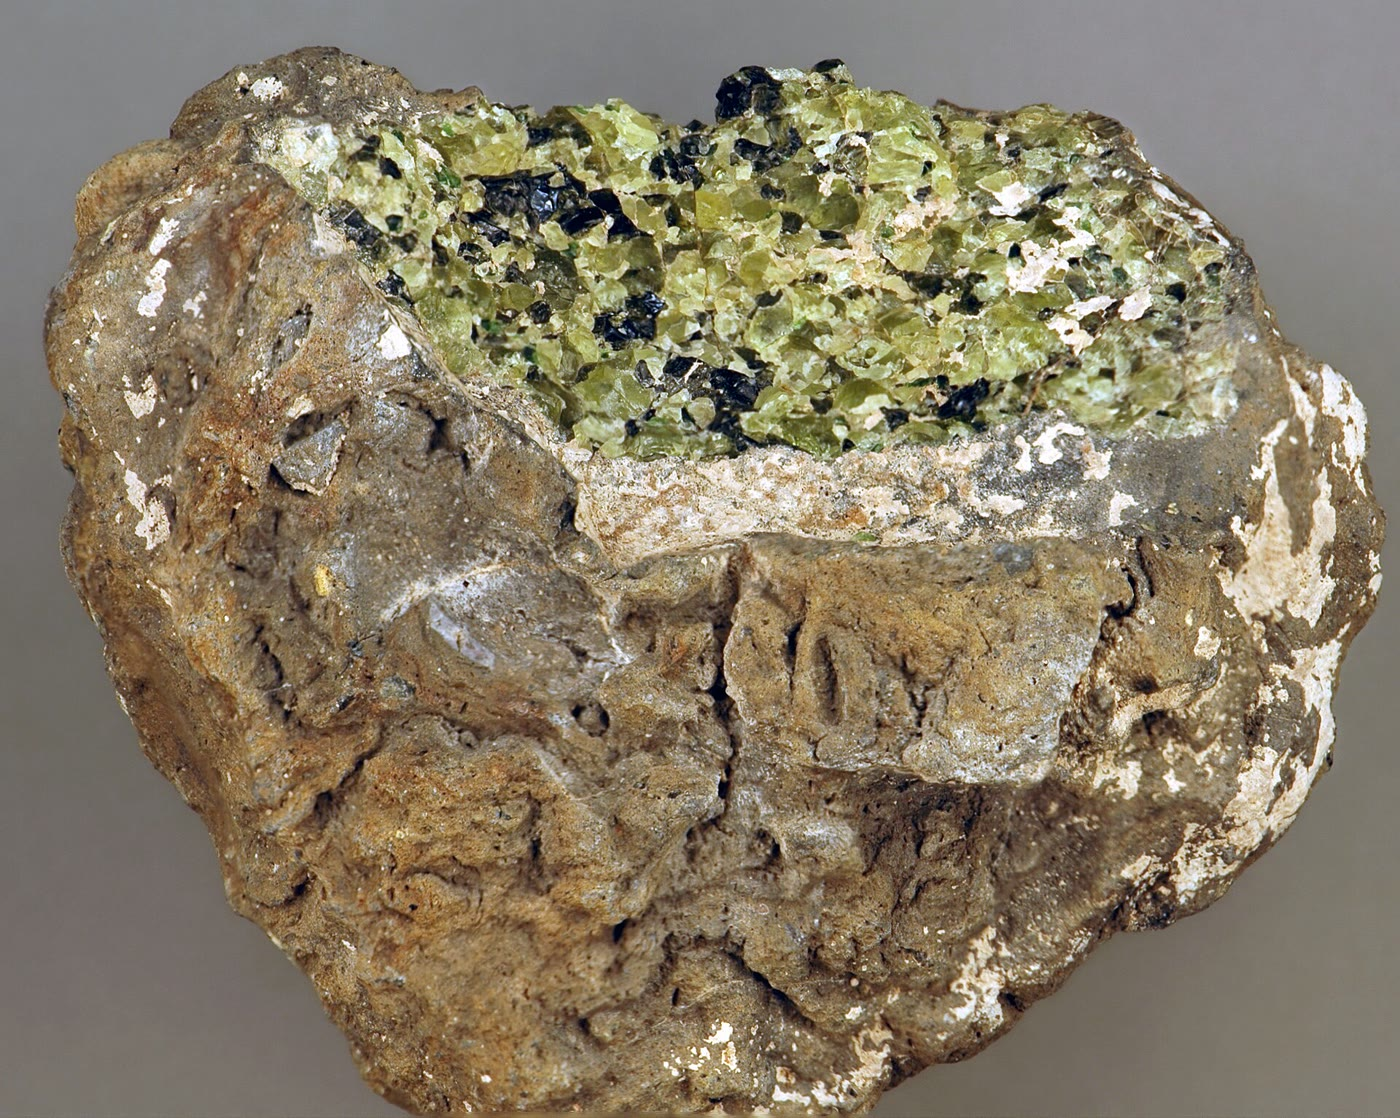
\includegraphics[width=\linewidth]{images/book4/b2-lherzolite-xenolith.jpg}
\end{minipage}\hfill
\begin{minipage}{0.48\linewidth}
{\small Un nódulo de peridotita del manto (lherzolita) en una lava basáltica de
Kilbourne Hole, Nuevo México, de \qty{7.4}{cm} en su parte más ancha: olivino
verde amarillento con piroxeno oscuro. La lava lo arrancó del manto superior y lo llevó
a la superficie. James St.~John, CC BY 2.0.}
\end{minipage}
\end{omfigure}

La figura siguiente compara esta Tierra silicatada con las \omterm{def:b2:elements-in-the-earth:ci}{condritas CI}, elemento por
elemento, frente a la \omterm{def:b2:planet-formation-meteorites:condensation}{temperatura de condensación} del capítulo anterior. Clasifica
los elementos como ningún otro dato puede hacerlo. Los \omterm{def:b2:elements-in-the-earth:goldschmidt}{elementos litófilos}
refractarios, desde el circonio y las \omterm{def:b2:elements-in-the-earth:ree}{tierras raras} hasta el estroncio y el bario, están todos
al mismo nivel, a menos de un veinte por ciento unos de otros: la Tierra silicatada
los conservó todos en sus proporciones condríticas. Los \omterm{def:b2:elements-in-the-earth:goldschmidt}{elementos litófilos} volátiles
caen con su \omterm{def:b2:planet-formation-meteorites:condensation}{temperatura de condensación}: hay en ella cerca de una quinta parte del potasio
y del sodio, una décima del rubidio, una centésima del cloro y unas pocas
milésimas del bromo y del yodo. Los \omterm{def:b2:elements-in-the-earth:goldschmidt}{elementos siderófilos} están muy por debajo de todo \omterm{def:b2:elements-in-the-earth:goldschmidt}{elemento litófilo}
de la misma volatilidad: la Tierra silicatada contiene una séptima parte de lo que le corresponde de
hierro, una treceava parte del níquel y unas tres milésimas de los
metales del grupo del platino y del oro. Estos se fueron al núcleo. Los \omterm{def:b2:elements-in-the-earth:goldschmidt}{elementos calcófilos},
la mayoría también volátiles, están empobrecidos por ambas razones.

\begin{omfigure}
\centering
\begin{tikzpicture}
\begin{axis}[omrecord, width=0.95\linewidth, height=8.2cm, ymode=log,
  xmin=500, xmax=1800, ymin=8e-4, ymax=3, x dir=reverse,
  xlabel={temperatura de condensación al 50 por ciento a \qty{e-4}{bar} (K)},
  ylabel={$(X/\mathrm{Mg})_{\mathrm{BSE}}\,/\,(X/\mathrm{Mg})_{\mathrm{CI}}$},
  legend pos=south west, legend cell align=left, legend style={font=\scriptsize},
  tick label style={font=\scriptsize}, label style={font=\small},
  scaled x ticks=false, xticklabel style={/pgf/number format/1000 sep={}}]
\addplot[black!40, dashed, domain=500:1800, samples=2, forget plot] {1};
\addplot[only marks, mark=*, mark size=1.6pt, brown!70!black]
  table[x=T, y=ratio] {figdata/out/bachelor-2-geochem-volat-lith.dat};
\addlegendentry{litófilos}
\addplot[only marks, mark=square*, mark size=1.6pt, blue!60!black]
  table[x=T, y=ratio] {figdata/out/bachelor-2-geochem-volat-sid.dat};
\addlegendentry{siderófilos}
\addplot[only marks, mark=triangle*, mark size=2pt, orange!80!black]
  table[x=T, y=ratio] {figdata/out/bachelor-2-geochem-volat-chal.dat};
\addlegendentry{calcófilos}
\node[font=\tiny, brown!50!black, anchor=south] at (axis cs:1600,1.35)
  {Zr, Hf, Al, Sc, Y, Th, U, Ti, Ca, Sr, Ba, tierras raras};
\begin{scope}[font=\tiny, brown!50!black]
\node[anchor=west] at (axis cs:1328,1.0) {Mg};
\node[anchor=north] at (axis cs:1310,0.80) {Si};
\node[anchor=west] at (axis cs:1150,0.23) {Mn};
\node[anchor=south] at (axis cs:1142,0.47) {Li};
\node[anchor=south] at (axis cs:1010,0.195) {K};
\node[anchor=north] at (axis cs:958,0.22) {Na};
\node[anchor=north] at (axis cs:908,0.175) {B};
\node[anchor=north] at (axis cs:800,0.116) {Rb};
\node[anchor=south] at (axis cs:734,0.175) {F};
\node[anchor=west] at (axis cs:795,0.0477) {Cs};
\node[anchor=west] at (axis cs:944,0.0102) {Cl};
\node[anchor=north] at (axis cs:546,0.0061) {Br};
\node[anchor=south] at (axis cs:535,0.0088) {I};
\end{scope}
\begin{scope}[font=\tiny, blue!50!black]
\node[anchor=west] at (axis cs:1325,0.144) {Fe};
\node[anchor=east] at (axis cs:1364,0.0775) {Ni};
\node[anchor=west] at (axis cs:1342,0.088) {Co};
\node[anchor=west] at (axis cs:1780,0.137) {W};
\node[anchor=south] at (axis cs:1590,0.0206) {Mo};
\node[anchor=north] at (axis cs:883,0.0139) {Ge};
\node[anchor=north] at (axis cs:1500,0.0026) {Re, Os, Ir, Ru, Pt, Pd};
\node[anchor=north] at (axis cs:1060,0.0026) {Au};
\end{scope}
\begin{scope}[font=\tiny, orange!60!black]
\node[anchor=west] at (axis cs:1030,0.0993) {Cu};
\node[anchor=north] at (axis cs:996,0.0167) {Ag};
\node[anchor=south] at (axis cs:726,0.0746) {Zn};
\node[anchor=south] at (axis cs:704,0.0325) {Sn};
\node[anchor=east] at (axis cs:735,0.0246) {Pb};
\node[anchor=west] at (axis cs:648,0.0249) {Cd};
\node[anchor=east] at (axis cs:715,0.0022) {Te};
\node[anchor=north] at (axis cs:690,0.0016) {Se};
\node[anchor=west] at (axis cs:660,0.0019) {S};
\end{scope}
\end{axis}
\end{tikzpicture}
\par\smallskip{\small La Tierra silicatada comparada con las \omterm{def:b2:elements-in-the-earth:ci}{condritas CI}: para cada elemento $X$, la
razón $X/\mathrm{Mg}$ en la \omterm{def:b2:elements-in-the-earth:bse}{Tierra silicatada global} dividida por la misma razón en las \omterm{def:b2:elements-in-the-earth:ci}{condritas
CI}, frente a la \omterm{def:b2:planet-formation-meteorites:condensation}{temperatura de condensación} al 50 por ciento (lo caliente a la izquierda).
Los \omterm{def:b2:elements-in-the-earth:goldschmidt}{elementos litófilos} refractarios son condríticos entre sí; los volátiles
se empobrecen al bajar la \omterm{def:b2:planet-formation-meteorites:condensation}{temperatura de condensación}; los siderófilos y
calcófilos se empobrecen mucho más. Datos: McDonough y Sun (1995);
Lodders (2003).}
\end{omfigure}
% ledger: ms95:pm-trace, lodders:ci-table, lodders:tc-table, lodders:tc-more

Los \omterm{def:b2:elements-in-the-earth:goldschmidt}{elementos litófilos} refractarios están un 15 por ciento por encima del magnesio. Ambos
no pueden ser exactamente condríticos: o la Tierra ganó \omterm{def:b2:elements-in-the-earth:volatility}{elementos refractarios},
o perdió un poco de magnesio, o el magnesio del modelo está
subestimado (\cref{exo:b2:elements-in-the-earth:12}). El silicio, con 0.83, se queda aún más lejos del
nivel refractario; parte del silicio que falta puede estar en el núcleo (problema).

Los \omterm{def:b2:elements-in-the-earth:goldschmidt}{elementos siderófilos} de la Tierra silicatada, combinados con una Tierra global condrítica,
pesan el núcleo. Supóngase que la Tierra global tiene la razón CI $r_X = X/\mathrm{Mg}$
para un \omterm{def:b2:elements-in-the-earth:goldschmidt}{elemento siderófilo} $X$, y que el núcleo contiene una concentración $c_X$ de él
pero nada de magnesio.

\begin{proposition}[Fracción másica del núcleo a partir de una razón condrítica]
\label{prop:b2:elements-in-the-earth:core}
Sean $x$ la fracción másica del núcleo, $C_X$ y $C_{\mathrm{Mg}}$ las
concentraciones de $X$ y de magnesio en la Tierra silicatada, y $c_X$ la de $X$ en
el núcleo. Si la Tierra tiene la razón condrítica $r_X$, entonces
\[
  \frac{x}{1-x} = \frac{r_X C_{\mathrm{Mg}} - C_X}{c_X}.
\]
\end{proposition}

\begin{proof}
Una masa $M$ de Tierra contiene $(1-x)MC_X + xMc_X$ de $X$ y $(1-x)MC_{\mathrm{Mg}}$ de
magnesio. Su cociente es $r_X$:
$(1-x)C_X + xc_X = r_X(1-x)C_{\mathrm{Mg}}$. Dividiendo por $(1-x)c_X$ se obtiene el
resultado.
\end{proof}

Con el hierro, $r_{\mathrm{Fe}} = \num{182800}/\num{95870} = 1.907$ en las \omterm{def:b2:elements-in-the-earth:ci}{condritas CI}, un
22.8 por ciento de magnesio y un 6.26 por ciento de hierro en la Tierra silicatada, y un 85.5 por
ciento de hierro en un núcleo modelo, la proposición da $x/(1-x) = 0.435$, un núcleo del 30
por ciento de la masa de la Tierra. La sismología, integrando la densidad del
modelo terrestre de referencia, da un 32.5 por ciento. La coincidencia dentro de una décima
apoya la imagen de una Tierra condrítica cuyo hierro está sobre todo en el núcleo; la
diferencia mide cuánto se aparta la razón hierro/magnesio de la Tierra de la
condrítica (problema). El mismo balance dice dónde está cada elemento de la Tierra
(figura siguiente): casi todo su platino, su iridio y su oro, y la mayor parte de su hierro,
su níquel y su azufre, están en el núcleo.
% ledger: lodders:ci-table, ms95:pm-trace, mcd03:core, data:prem

\begin{omfigure}
\centering
\begin{tikzpicture}
\begin{axis}[omrecord, xbar, width=0.8\linewidth, height=6.4cm, bar width=5pt,
  xmin=0, xmax=100, ymin=0.4, ymax=14.6, y dir=reverse,
  ytick={1,...,14}, yticklabels from table={figdata/out/bachelor-2-geochem-budget.dat}{el},
  xlabel={proporción del inventario terrestre contenida en el núcleo (por ciento)},
  tick label style={font=\scriptsize}, label style={font=\small},
  nodes near coords, nodes near coords align={horizontal},
  every node near coord/.append style={font=\tiny, /pgf/number format/fixed,
    /pgf/number format/precision=1}]
\addplot[fill=blue!35!gray!50, draw=black!60]
  table[x=share, y=idx] {figdata/out/bachelor-2-geochem-budget.dat};
\end{axis}
\end{tikzpicture}
\par\smallskip{\small Dónde están los elementos de la Tierra: la proporción de cada elemento contenida en
el núcleo, a partir de una composición modelo del núcleo, del \omterm{def:b2:elements-in-the-earth:bse}{manto primitivo} y de un núcleo del 32.5
por ciento de la masa de la Tierra. Datos: McDonough (2003); McDonough y Sun (1995);
modelo terrestre de referencia.}
\end{omfigure}
% ledger: mcd03:core, ms95:pm-trace, data:prem

\section{El manto y las cortezas}

La Tierra silicatada está dividida desde su formación en un manto y dos
tipos de corteza. La corteza oceánica se forma por fusión del manto bajo las
dorsales oceánicas; la corteza continental, por una larga historia de fusión sobre las
zonas de subducción, de retrabajo y de erosión (capítulos posteriores). Dos fundidos de referencia
del manto sirven de base a la discusión.

\begin{definition}[Basalto de dorsal oceánica, basalto de isla oceánica]
\label{def:b2:elements-in-the-earth:morb-oib}
Un \emph{basalto de dorsal oceánica}\index{basalto de dorsal oceánica} (MORB) es un basalto
emitido en una dorsal oceánica, la roca de la parte superior de la corteza oceánica. Un
\emph{basalto de isla oceánica}\index{basalto de isla oceánica} (OIB) es un basalto emitido
en un volcán oceánico alejado de los límites de placa, como los de Hawái,
atribuido por lo común a una pluma del manto (volumen de primer año).
\end{definition}

El MORB medio de la tabla siguiente es una media global construida a partir de 771 segmentos
de dorsal, cada segmento ponderado por su longitud y su velocidad de expansión, de modo que la
media representa la corteza que producen las dorsales. La columna del OIB
es una sola roca: el material de referencia basáltico BHVO-2, tomado en 1995
de una lava que desbordó el cráter Halemaumau del Kilauea, Hawái, en 1919,
y analizado por muchos laboratorios, de modo que la mayoría de sus \omterm{def:b2:elements-in-the-earth:ree}{tierras raras} se conocen con
cerca de un uno por ciento. La corteza continental superior es una media estimada a partir de
rocas y sedimentos de superficie.
% ledger: gale13:allmorb, usgs:bhvo2-origin, usgs:bhvo2-major, rg14:crust

\begin{table}[h]
\centering
\small
\begin{tabular}{lrrrr}
\hline
óxido (\% en masa) & \omterm{def:b2:elements-in-the-earth:bse}{manto primitivo} & MORB & OIB (BHVO-2) & corteza cont.\ superior\\
\hline
\ce{SiO2} & 45.0 & 50.47 & 49.60 & 66.6\\
\ce{TiO2} & 0.201 & 1.68 & 2.731 & 0.64\\
\ce{Al2O3} & 4.45 & 14.70 & 13.44 & 15.4\\
FeO (total) & 8.05 & 10.43 & 11.15 & 5.04\\
MnO & 0.135 & 0.184 & 0.1690 & 0.10\\
MgO & 37.8 & 7.58 & 7.257 & 2.48\\
CaO & 3.55 & 11.39 & 11.40 & 3.59\\
\ce{Na2O} & 0.36 & 2.79 & 2.219 & 3.27\\
\ce{K2O} & 0.029 & 0.160 & 0.5130 & 2.80\\
\ce{P2O5} & 0.021 & 0.184 & 0.2685 & 0.15\\
\hline
\end{tabular}
\caption{Composiciones en elementos mayores de cuatro reservorios. BHVO-2 da su hierro como
\ce{Fe2O3} (12.39 por ciento), aquí convertido a FeO. Datos: McDonough y Sun
(1995); Gale y colaboradores (2013); hoja informativa del USGS sobre BHVO-2; Rudnick y
Gao (2014).}
\label{tab:b2:elements-in-the-earth:majors}
\end{table}
% ledger: ms95:pm-oxides, gale13:allmorb, usgs:bhvo2-major, rg14:crust

Leída en horizontal, la tabla cuenta la historia de la fusión. El manto es una peridotita
rica en magnesio, con casi un 38 por ciento de MgO y menos de un 5 por ciento de \ce{Al2O3} y de CaO.
Sus fundidos, los basaltos, contienen cinco veces menos magnesio y tres veces más
calcio y aluminio: los elementos que entran fácilmente en el fundido abandonan el manto
primero. El potasio, el sodio y el titanio son aún más ricos en los fundidos respecto
al manto, y el potasio es el más rico de todos en la corteza continental,
casi cien veces su concentración en el \omterm{def:b2:elements-in-the-earth:bse}{manto primitivo}. El silicio aumenta
poco del manto a los basaltos, y mucho más en la corteza
continental, cuya media se acerca a la de una granodiorita.

\section{Elementos en trazas}

Diez óxidos forman cerca del 99 por ciento de cada roca de la tabla anterior. Los demás elementos,
presentes en partes por millón, siguen los mismos procesos que los mayores, pero
son mucho más sensibles a ellos.

\begin{definition}[Elemento en trazas]\label{def:b2:elements-in-the-earth:trace}
Un \emph{elemento en trazas}\index{elemento en trazas} de una roca es un elemento cuya
concentración está, por convenio, por debajo del 0.1 por ciento en masa (\qty{1000}{ppm}).
Los elementos en trazas rara vez forman minerales propios; sustituyen a elementos
mayores en los sitios de las redes cristalinas.
\end{definition}

Un \omterm{def:b2:elements-in-the-earth:trace}{elemento en trazas} está tan diluido que su propia concentración no modifica los
cristales ni el fundido: su distribución entre ellos es entonces un simple cociente,
independiente de su concentración en un intervalo amplio.

\begin{definition}[Coeficiente de reparto mineral--fundido; elementos compatibles e
incompatibles]\label{def:b2:elements-in-the-earth:partition}
El \emph{coeficiente de reparto mineral--fundido}\index{coeficiente de reparto mineral--fundido}
de un elemento en un mineral es el cociente de sus concentraciones en el
mineral y en un fundido silicatado en equilibrio con él,
$D = C_{\mathrm{mineral}}/C_{\mathrm{melt}}$. Para una roca de varios minerales de
fracciones másicas $x_i$, el \emph{coeficiente de reparto global} es
$\bar D = C_{\mathrm{rock}}/C_{\mathrm{melt}}$. Un elemento es un
\emph{elemento compatible}\index{elemento compatible} en una roca si $\bar D > 1$,
y un \emph{elemento incompatible}\index{elemento incompatible} si $\bar D < 1$.
\end{definition}

\begin{proposition}[Coeficiente de reparto global]
\label{prop:b2:elements-in-the-earth:bulk-d}
Si cada mineral de la roca está en equilibrio con el mismo fundido, el coeficiente
de reparto global es la media de los coeficientes de los minerales ponderada por
las fracciones másicas: $\bar D = \sum_i x_i D_i$.
\end{proposition}

\begin{proof}
La roca contiene $C_{\mathrm{rock}} = \sum_i x_i C_i$, y cada mineral
$C_i = D_i C_{\mathrm{melt}}$. Dividiendo por $C_{\mathrm{melt}}$ se obtiene el resultado.
\end{proof}

Que un ion quepa en un sitio depende de su radio y de su carga. Un ion cercano en
radio y en carga al ion mayor del sitio, como \ce{Ni^2+} respecto a \ce{Mg^2+} en el
olivino, entra con facilidad y es compatible. Un ion mucho mayor, como
\ce{Rb+} o \ce{Ba^2+}, o con más carga, como \ce{Zr^4+} o
\ce{Nb^5+}, deforma la red y es expulsado al fundido: es
incompatible en los minerales del manto. Dos grupos de \omterm{def:b2:elements-in-the-earth:partition}{elementos incompatibles}
se comportan de manera distinta más adelante, cuando interviene el agua.

\begin{definition}[Elementos litófilos de ion grande y de alto potencial iónico]
\label{def:b2:elements-in-the-earth:lile-hfse}
Los \emph{elementos litófilos de ion grande}\index{elemento litófilo de ion grande}
(LILE) son \omterm{def:b2:elements-in-the-earth:partition}{elementos incompatibles} de iones grandes y carga baja, $+1$ o $+2$:
potasio, rubidio, cesio, estroncio, bario. Los
\emph{elementos de alto potencial iónico}\index{elemento de alto potencial iónico} (HFSE)
son \omterm{def:b2:elements-in-the-earth:partition}{elementos incompatibles} de iones pequeños y muy cargados, $+4$ o $+5$:
circonio, hafnio, niobio, tántalo, titanio.
\end{definition}

Los LILE se disuelven fácilmente en los fluidos ricos en agua; los HFSE apenas lo hacen. Una roca
alterada por el agua o un fundido que heredó fluidos, como sobre las zonas de subducción,
llevan por tanto LILE con pocos HFSE.

\begin{definition}[Tierras raras]\label{def:b2:elements-in-the-earth:ree}
Las \emph{tierras raras}\index{tierras raras} (REE) son los quince
lantánidos, del lantano al lutecio; el prometio no tiene isótopo estable. Todas
son litófilas y refractarias, casi todas trivalentes, y su radio iónico
disminuye de forma regular del lantano al lutecio; el europio puede ser también divalente en
fundidos reducidos.
\end{definition}

Como las \omterm{def:b2:elements-in-the-earth:ree}{tierras raras} difieren de forma gradual en el radio y en nada más,
se fraccionan de forma gradual: las ligeras, del lantano al samario, son las menos
compatibles; las pesadas, del gadolinio al lutecio, encajan mejor en algunos
minerales, sobre todo en el granate (figura siguiente). En una roca con granate, las \omterm{def:b2:elements-in-the-earth:ree}{tierras raras}
pesadas se vuelven compatibles: un fundido de esa roca es rico en \omterm{def:b2:elements-in-the-earth:ree}{tierras raras} ligeras y
pobre en las pesadas.

\begin{omfigure}
\centering
\begin{tikzpicture}
\begin{axis}[omrecord, width=0.78\linewidth, height=6.4cm, ymode=log,
  xmin=0.6, xmax=9.4, ymin=5e-4, ymax=20,
  xtick={1,...,9}, xticklabels from table={figdata/out/bachelor-2-geochem-dvals.dat}{el},
  ylabel={coeficiente de reparto $D$}, legend pos=south east,
  legend cell align=left, legend style={font=\scriptsize},
  tick label style={font=\scriptsize}, label style={font=\small}]
\addplot[black!40, dashed, domain=0.6:9.4, samples=2, forget plot] {1};
\addplot[thick, green!45!black, mark=*] table[x=idx, y=cpx] {figdata/out/bachelor-2-geochem-dvals.dat};
\addlegendentry{clinopiroxeno}
\addplot[thick, red!70!black, mark=square*] table[x=idx, y=gar] {figdata/out/bachelor-2-geochem-dvals.dat};
\addlegendentry{granate}
\addplot[thick, olive!70!black, mark=triangle*] table[x=idx, y=ol] {figdata/out/bachelor-2-geochem-dvals.dat};
\addlegendentry{olivino + ortopiroxeno + espinela}
\addplot[very thick, black, mark=diamond*] table[x=idx, y=bulk] {figdata/out/bachelor-2-geochem-dvals.dat};
\addlegendentry{roca total (65/18/17 por ciento)}
\node[font=\scriptsize, anchor=south west] at (axis cs:0.7,1) {compatible};
\node[font=\scriptsize, anchor=north west] at (axis cs:0.7,1) {incompatible};
\end{axis}
\end{tikzpicture}
\par\smallskip{\small \omterm{def:b2:elements-in-the-earth:partition}{Coeficientes de reparto mineral--fundido} de las \omterm{def:b2:elements-in-the-earth:ree}{tierras raras} para el
clinopiroxeno, el granate y una mezcla de olivino, ortopiroxeno y espinela, y el
coeficiente global de una piroxenita con granate de un 65 por ciento de clinopiroxeno, un 18 por
ciento de granate y un 17 por ciento de los demás minerales (proposición anterior). El granate
hace compatibles las \omterm{def:b2:elements-in-the-earth:ree}{tierras raras} pesadas. Datos: Budahn (1991).}
\end{omfigure}
% ledger: budahn91:d-ree, budahn91:modes

\section{Diagramas normalizados}

Las abundancias de elementos vecinos difieren en factores grandes por la
historia nuclear de la materia: los elementos de número atómico par son más abundantes que
sus vecinos impares, como muestra la columna CI de las \omterm{def:b2:elements-in-the-earth:ree}{tierras raras} (lantano 0.232,
cerio 0.621, praseodimio 0.0928 ppm). Representadas en bruto, las \omterm{def:b2:elements-in-the-earth:ree}{tierras raras} de una roca forman un
diente de sierra que oculta su historia geológica. Dividir por una referencia lo elimina.
% ledger: lodders:ci-table

\begin{definition}[Diagrama normalizado]\label{def:b2:elements-in-the-earth:normalised}
Un \emph{diagrama normalizado}\index{diagrama normalizado} representa, para una serie de
elementos en un orden fijo, la concentración en una muestra dividida por la de una
referencia, $X_N = C_X/C_X^{\mathrm{ref}}$, en escala logarítmica. Las \omterm{def:b2:elements-in-the-earth:ree}{tierras raras}
se normalizan a las \omterm{def:b2:elements-in-the-earth:ci}{condritas CI} en el orden del número atómico; un conjunto más largo de
\omterm{def:b2:elements-in-the-earth:partition}{elementos incompatibles}, llamado a menudo diagrama de araña, se normaliza al
\omterm{def:b2:elements-in-the-earth:bse}{manto primitivo} y se ordena por incompatibilidad decreciente en la fusión del manto.
\end{definition}

Una muestra con las mismas proporciones que la referencia se representa como una línea horizontal;
su altura da el enriquecimiento. Una pendiente indica un fraccionamiento entre elementos
ligeros y pesados, medido por una razón como $(\mathrm{La}/\mathrm{Yb})_N$. Un
único elemento fuera de la línea es una anomalía.

\begin{proposition}[Anomalía de europio]\label{prop:b2:elements-in-the-earth:normalised}
En un \omterm{def:b2:elements-in-the-earth:normalised}{diagrama normalizado} en el que el perfil es una recta en
$\log X_N$ entre el samario y el gadolinio, el valor esperado para el europio, que
está en el punto medio, es $\mathrm{Eu}^* = \sqrt{\mathrm{Sm}_N\,\mathrm{Gd}_N}$. La
\emph{anomalía de europio}\index{anomalía de europio} es
$\mathrm{Eu}/\mathrm{Eu}^* = \mathrm{Eu}_N/\sqrt{\mathrm{Sm}_N\,\mathrm{Gd}_N}$:
por debajo de 1 es negativa, por encima de 1 positiva.
\end{proposition}

\begin{proof}
El samario, el europio y el gadolinio son consecutivos, a pasos iguales a lo largo del eje.
Una recta en $\log X_N$ toma en el punto medio la media de los valores extremos:
$\log \mathrm{Eu}^* = \tfrac12(\log \mathrm{Sm}_N + \log \mathrm{Gd}_N)$, el
logaritmo de la media geométrica.
\end{proof}

El europio es la única tierra rara que puede ser divalente. \ce{Eu^2+} tiene casi el
radio de \ce{Ca^2+} y de \ce{Sr^2+}, de modo que el feldespato plagioclasa lo admite donde
rechaza las \omterm{def:b2:elements-in-the-earth:ree}{tierras raras} trivalentes. Un fundido del que ha cristalizado plagioclasa
tiene una anomalía negativa; la roca rica en plagioclasa que queda atrás, una positiva.

\begin{omfigure}
\centering
\begin{tikzpicture}
\begin{axis}[omrecord, width=0.8\linewidth, height=6.4cm, ymode=log,
  xmin=0.6, xmax=13.4, ymin=5, ymax=250,
  xtick={1,...,13}, xticklabels from table={figdata/out/bachelor-2-geochem-ree.dat}{el},
  ylabel={muestra / condrita CI}, legend pos=north east, legend cell align=left,
  legend style={font=\scriptsize}, tick label style={font=\scriptsize},
  label style={font=\small}]
\addplot[thick, blue!70!black, mark=*] table[x=idx, y=morb] {figdata/out/bachelor-2-geochem-ree.dat};
\addlegendentry{MORB medio}
\addplot[thick, red!70!black, mark=square*] table[x=idx, y=oib] {figdata/out/bachelor-2-geochem-ree.dat};
\addlegendentry{OIB (BHVO-2, Hawái)}
\addplot[thick, brown!70!black, mark=triangle*] table[x=idx, y=ucc] {figdata/out/bachelor-2-geochem-ree.dat};
\addlegendentry{corteza continental superior}
\end{axis}
\end{tikzpicture}
\par\smallskip{\small Perfiles de \omterm{def:b2:elements-in-the-earth:ree}{tierras raras} normalizados a las \omterm{def:b2:elements-in-the-earth:ci}{condritas CI} (sin el tulio, a
falta de un valor para el MORB). El MORB medio es plano, algo más pobre en las \omterm{def:b2:elements-in-the-earth:ree}{tierras raras}
ligeras; el basalto hawaiano está enriquecido en ellas; la corteza superior está muy
enriquecida en ellas, con una \omterm{prop:b2:elements-in-the-earth:normalised}{anomalía de europio} negativa. Datos: Gale y colaboradores
(2013); hoja del USGS sobre BHVO-2; Rudnick y Gao; Lodders (2003).}
\end{omfigure}
% ledger: gale13:allmorb, usgs:bhvo2-trace, rg03:ucc-trace, lodders:ci-table

Los tres perfiles de la figura anterior se leen como tres historias. El MORB medio
está unas 25 veces por encima de la \omterm{def:b2:planet-formation-meteorites:chondrule}{condrita}, casi plano, con $(\mathrm{La}/\mathrm{Sm})_N
= 0.85$: su fuente mantélica ya había perdido parte de sus elementos más incompatibles
en fundidos anteriores, entre ellos la corteza continental. El basalto hawaiano está
enriquecido en las \omterm{def:b2:elements-in-the-earth:ree}{tierras raras} ligeras, $(\mathrm{La}/\mathrm{Yb})_N = 5.4$, y sus
\omterm{def:b2:elements-in-the-earth:ree}{tierras raras} pesadas están por debajo de las del MORB: procede de un grado de fusión
menor, en el que quedó atrás granate que retenía las pesadas. La corteza
continental superior está enriquecida más de cien veces en lantano, con
$(\mathrm{La}/\mathrm{Yb})_N = 10.9$ y $\mathrm{Eu}/\mathrm{Eu}^* = 0.72$: es
el producto de fusiones repetidas, y su déficit de europio es coherente con
plagioclasa que quedó atrás en la corteza profunda.

\begin{omfigure}
\centering
\begin{tikzpicture}
\begin{axis}[omrecord, width=\linewidth, height=6.6cm, ymode=log,
  xmin=0.5, xmax=27.5, ymin=1, ymax=400,
  xtick={1,...,27}, xticklabels from table={figdata/out/bachelor-2-geochem-spider.dat}{el},
  ylabel={muestra / manto primitivo}, legend pos=north east, legend cell align=left,
  legend style={font=\scriptsize}, tick label style={font=\scriptsize},
  label style={font=\small}]
\addplot[thick, blue!70!black, mark=*, mark size=1.4pt] table[x=idx, y=morb] {figdata/out/bachelor-2-geochem-spider.dat};
\addlegendentry{MORB medio}
\addplot[thick, red!70!black, mark=square*, mark size=1.4pt] table[x=idx, y=oib] {figdata/out/bachelor-2-geochem-spider.dat};
\addlegendentry{OIB (BHVO-2)}
\addplot[thick, brown!70!black, mark=triangle*, mark size=1.6pt] table[x=idx, y=ucc] {figdata/out/bachelor-2-geochem-spider.dat};
\addlegendentry{corteza continental superior}
\end{axis}
\end{tikzpicture}
\par\smallskip{\small \omterm{def:b2:elements-in-the-earth:partition}{Elementos incompatibles} normalizados al \omterm{def:b2:elements-in-the-earth:bse}{manto primitivo}, del más
incompatible a la izquierda. La corteza continental muestra los LILE altos, los profundos
valles del niobio, el tántalo y el titanio y el pico del plomo heredados de la
fusión en zonas de subducción; el basalto hawaiano muestra una joroba en el niobio y el
tántalo. Potasio y titanio calculados a partir de los óxidos. Datos: los de la figura de
las \omterm{def:b2:elements-in-the-earth:ree}{tierras raras}; McDonough y Sun (1995).}
\end{omfigure}
% ledger: gale13:allmorb, usgs:bhvo2-trace, usgs:bhvo2-major, rg03:ucc-trace, ms95:pm-trace

El diagrama de araña anterior acentúa el contraste. En la corteza continental,
el niobio y el tántalo quedan muy por debajo de sus vecinos el torio y el lantano,
el titanio por debajo de sus vecinos, y el plomo muy por encima: $(\mathrm{Nb}/\mathrm{La})_N =
0.38$. En el basalto hawaiano la misma razón vale 1.17, y en el MORB medio
0.99. El perfil de la corteza es la firma de los fundidos sobre las zonas de subducción, donde
los fluidos llevaron los LILE y el plomo a la cuña del manto y dejaron atrás los HFSE
(capítulos posteriores); los \omterm{def:b2:elements-in-the-earth:morb-oib}{basaltos de isla oceánica} carecen de ella. El diagrama de araña de una sola muestra
puede por tanto distinguir una lava de arco de una lava de isla oceánica, o revelar un basalto
contaminado por corteza continental (\cref{exo:b2:elements-in-the-earth:11}).

\begin{inthelab}[De una roca a una lista de elementos en trazas]
\begin{minipage}[t]{0.6\linewidth}
\vspace{0pt}
Un geoquímico que quiere los \omterm{def:b2:elements-in-the-earth:trace}{elementos en trazas} de un basalto parte de unos cientos
de gramos de su interior más fresco, libre de corteza de alteración y de venas. La roca se
tritura y luego se muele hasta un polvo fino en un molino cuyo material no
contamine los elementos de interés. Una pequeña porción del polvo se
pone en disolución con ácidos, o se funde con un fundente, y la disolución se analiza por
espectrometría de masas con plasma de acoplamiento inductivo, que mide la mayoría de los
elementos del diagrama de araña a la vez. Con cada lote de muestras el
laboratorio analiza materiales de referencia de composición conocida, como el
basalto hawaiano BHVO-2: sus valores proceden de un estudio que combinó las medias de
muchos laboratorios, 132 de ellos para el lantano, y algunos, como los valores del
neodimio y del samario, por dilución isotópica, que cuenta los átomos de
un elemento frente a una cantidad añadida conocida de uno de sus isótopos. Si el resultado del laboratorio para el material de referencia está
dentro de la incertidumbre del valor aceptado, los resultados de las muestras desconocidas
se aceptan con él.
\end{minipage}\hfill
\begin{minipage}[t]{0.36\linewidth}
\vspace{0pt}
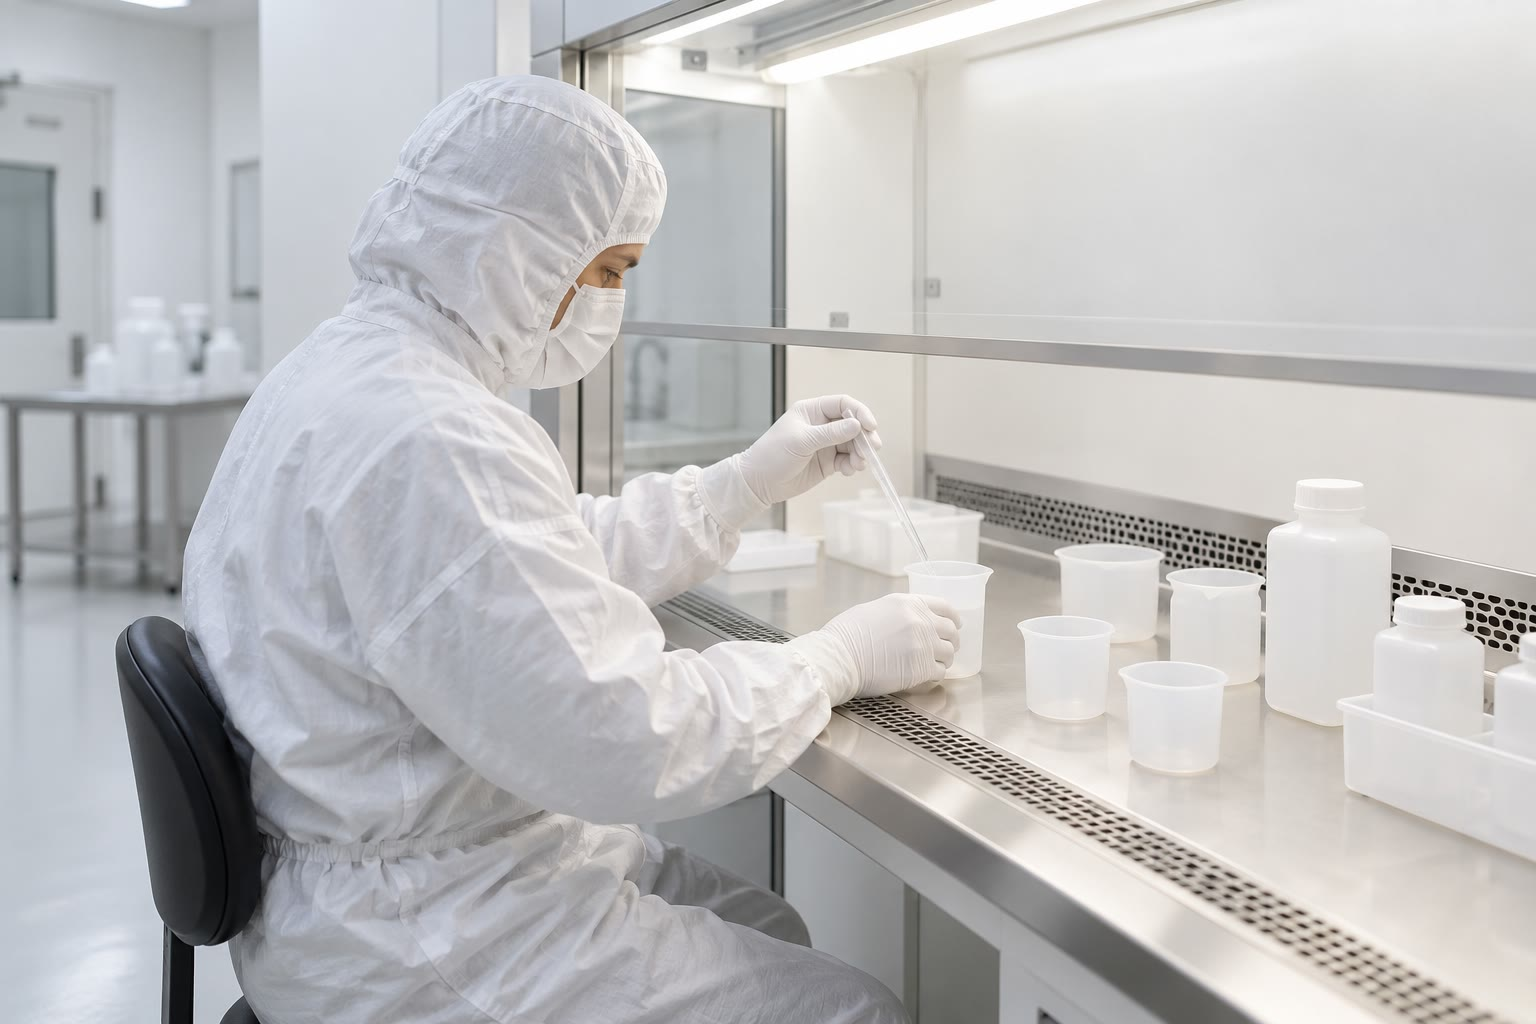
\includegraphics[width=\linewidth]{images/book4/ai/b2-clean-lab.jpg}

\smallskip
{\footnotesize Un técnico con traje de sala blanca en la campana de flujo laminar de un
laboratorio limpio de geoquímica (ilustración generada por IA).\par}
\end{minipage}
\end{inthelab}
% ledger: usgs:bhvo2-trace, usgs:bhvo2-origin

\section{Ejercicios}

\begin{exercise}[$\star$]\label{exo:b2:elements-in-the-earth:1}
El basalto BHVO-2 contiene un 0.5130 por ciento de \ce{K2O} y un 2.731 por ciento de \ce{TiO2}
en masa. Con las masas atómicas K 39.10, Ti 47.87 y O 16.00, calcúlense sus
contenidos en potasio y en titanio en ppm.
\end{exercise}

\begin{exercise}[$\star$]\label{exo:b2:elements-in-the-earth:2}
En la \omterm{def:b2:elements-in-the-earth:bse}{Tierra silicatada global}, las razones $(X/\mathrm{Mg})$ divididas por las razones CI
valen 1.16 para el aluminio, 0.22 para el sodio, 0.077 para el níquel y 0.0029 para el
iridio. Las \omterm{def:b2:planet-formation-meteorites:condensation}{temperaturas de condensación} de estos elementos son 1653, 958, 1353
y \qty{1603}{K}. Dese la clase de Goldschmidt de cada elemento y explíquese cada
empobrecimiento.
\end{exercise}

\begin{exercise}[$\star$]\label{exo:b2:elements-in-the-earth:3}
La corteza continental superior contiene \qty{31}{ppm} de lantano y \qty{2.0}{ppm}
de iterbio; las \omterm{def:b2:elements-in-the-earth:ci}{condritas CI}, 0.232 y \qty{0.163}{ppm}. Calcúlense los
valores normalizados a la \omterm{def:b2:planet-formation-meteorites:chondrule}{condrita} y $(\mathrm{La}/\mathrm{Yb})_N$. ¿Qué dice la
razón sobre la corteza?
\end{exercise}

\begin{exercise}[$\star$]\label{exo:b2:elements-in-the-earth:4}
La corteza continental superior contiene 4.7, 1.0 y \qty{4.0}{ppm} de samario,
europio y gadolinio; las \omterm{def:b2:elements-in-the-earth:ci}{condritas CI}, 0.145, 0.0546 y \qty{0.198}{ppm}.
Calcúlese $\mathrm{Eu}/\mathrm{Eu}^*$. ¿Qué mineral explica el resultado?
\end{exercise}

\begin{exercise}[$\star\star$]\label{exo:b2:elements-in-the-earth:5}
Una piroxenita con granate está formada por un 65 por ciento de clinopiroxeno, un 18 por ciento de granate y
un 17 por ciento de olivino, ortopiroxeno y espinela. Los coeficientes de reparto del
lantano son 0.058, 0.001 y 0.001, y los del lutecio 0.53, 5.8 y 0.18.
Calcúlense los coeficientes globales. ¿Qué elemento es compatible en la roca? ¿Qué
mineral contiene la mayor parte del lutecio de la roca?
\end{exercise}

\begin{exercise}[$\star\star$]\label{exo:b2:elements-in-the-earth:6}
La \omterm{def:b2:elements-in-the-earth:bse}{Tierra silicatada global} contiene un 22.8 por ciento de magnesio, \qty{2670}{ppm} de
sodio y \qty{1960}{ppm} de níquel; las \omterm{def:b2:elements-in-the-earth:ci}{condritas CI}, un 9.587 por ciento,
\qty{5010}{ppm} y \qty{10640}{ppm}. Calcúlense las razones normalizadas al Mg respecto a CI para
el sodio y el níquel. Ambos elementos condensan cerca de \qty{1000}{K} o por encima; ¿por qué está
más empobrecido el níquel?
\end{exercise}

\begin{exercise}[$\star\star$]\label{exo:b2:elements-in-the-earth:7}
Un clinopiroxeno cristaliza a partir de un fundido con la composición del MORB medio,
\qty{5.21}{ppm} de lantano y \qty{0.53}{ppm} de lutecio. Sus coeficientes de reparto
son 0.058 para el lantano y 0.53 para el lutecio. Calcúlense sus
contenidos en lantano y en lutecio, y el cociente entre $(\mathrm{La}/\mathrm{Lu})_N$
en el cristal y en el fundido (CI: La 0.232, Lu \qty{0.0237}{ppm}).
\end{exercise}

\begin{exercise}[$\star\star$]\label{exo:b2:elements-in-the-earth:8}
Normalizando al \omterm{def:b2:elements-in-the-earth:bse}{manto primitivo} (Nb \qty{0.658}{ppm}, La \qty{0.648}{ppm}),
calcúlese $(\mathrm{Nb}/\mathrm{La})_N$ para la corteza continental superior (Nb 12,
La \qty{31}{ppm}), el basalto hawaiano (18.10, \qty{15.20}{ppm}) y el MORB medio
(5.24, \qty{5.21}{ppm}). ¿Cuál de ellos lleva la firma de las zonas de subducción?
\end{exercise}

\begin{exercise}[$\star\star$]\label{exo:b2:elements-in-the-earth:9}
El potasio y el uranio son ambos muy incompatibles. Calcúlese la razón másica K/U en
el \omterm{def:b2:elements-in-the-earth:bse}{manto primitivo} (K \qty{240}{ppm}, U \qty{0.0203}{ppm}), en el MORB medio
(\qty{0.160}{\percent} de \ce{K2O}, U \qty{0.119}{ppm}) y en la corteza continental
superior (\qty{2.80}{\percent} de \ce{K2O}, U \qty{2.7}{ppm}), usando
$\mathrm{K}/\ce{K2O} = 0.830$ en masa. ¿Qué significa que la razón sea casi constante,
y por qué es útil K/U para estimar el potasio de un planeta?
\end{exercise}

\begin{exercise}[$\star\star\star$]\label{exo:b2:elements-in-the-earth:10}
Una pequeña cantidad de fundido está en equilibrio con la piroxenita con granate del ejercicio
5. Demuéstrese que, para dos elementos, el cociente
$(C_1/C_2)_{\mathrm{melt}}/(C_1/C_2)_{\mathrm{rock}}$ es igual a
$\bar D_2/\bar D_1$. Calcúlese para el lantano y el lutecio, y explíquese por qué los
fundidos de un manto con granate tienen perfiles de \omterm{def:b2:elements-in-the-earth:ree}{tierras raras} muy inclinados.
\end{exercise}

\begin{exercise}[$\star\star\star$]\label{exo:b2:elements-in-the-earth:11}
Un MORB medio (Th \qty{0.404}{ppm}, Nb \qty{5.24}{ppm}) asimila corteza continental
superior (Th \qty{10.5}{ppm}, Nb \qty{12}{ppm}): una fracción másica $f$ de
corteza se mezcla con $1-f$ de basalto. Demuéstrese que las concentraciones de la mezcla son
lineales en $f$ pero que su razón Th/Nb no lo es. Hállese el $f$ con el que Th/Nb alcanza
0.2, y la razón para $f = 0.1$.
\end{exercise}

\begin{exercise}[$\star\star\star$]\label{exo:b2:elements-in-the-earth:12}
Retirar agua, carbono o un núcleo metálico que no contenga ni aluminio ni
magnesio no cambia la razón Al/Mg del resto: demuéstrese. En la \omterm{def:b2:elements-in-the-earth:bse}{Tierra silicatada
global}, $(\mathrm{Al}/\mathrm{Mg})$ vale 1.16 veces el valor CI. Si la
Tierra conservó todo su aluminio, ¿qué fracción de su magnesio condrítico
falta en la Tierra silicatada? Con la razón del silicio normalizada al Mg,
0.83, ¿qué fracción de su silicio condrítico faltaría con el mismo
supuesto?
\end{exercise}

\section{Problema: pesar el núcleo con una condrita}

\begin{problem}[{Problema de fin de semana --- reconstruir la Tierra global a partir de las condritas
CI, del manto y del núcleo, y pesar el núcleo}]
\label{pb:b2:elements-in-the-earth:1}
Una geoquímica planetaria quiere pesar el núcleo de la Tierra sin sismología,
solo con la química. Toma como material de partida las \omterm{def:b2:elements-in-the-earth:ci}{condritas CI} (Mg \qty{95870}{ppm},
Al 8500, Si \num{106500}, Fe \num{182800}, Ni
\qty{10640}{ppm}), el \omterm{def:b2:elements-in-the-earth:bse}{manto primitivo} para la Tierra silicatada (MgO 37.8, FeO
8.05, NiO 0.25 por ciento; Mg 22.8, Si 21.0 por ciento), y un núcleo modelo con un 85.5
por ciento de Fe, un 5.2 por ciento de Ni y un 6.0 por ciento de Si. Masas atómicas: Mg 24.31,
Si 28.09, Fe 55.85, Ni 58.69, O 16.00. Masa de la Tierra:
\qty{5.972e24}{kg}.

\medskip\noindent\textbf{Parte I --- El punto de partida condrítico.}
\begin{enumerate}
\item Calcúlense las razones másicas Fe/Mg, Ni/Mg, Si/Mg y Al/Mg de las \omterm{def:b2:elements-in-the-earth:ci}{condritas CI}.
\item Conviértase Fe/Si en una razón atómica. La espectroscopia de la fotosfera solar
da 0.81 átomos de hierro por átomo de silicio: ¿es razonable la comparación?
\item Las \omterm{def:b2:elements-in-the-earth:ci}{condritas CI} contienen un 2.1 por ciento de hidrógeno y un 3.5 por ciento de carbono, ligados en
minerales hidratados y compuestos orgánicos que la Tierra no conservó. ¿Por qué
no hace falta corregir las razones de la pregunta 1 de esta pérdida?
\item ¿Por qué es el magnesio un elemento de referencia adecuado para el problema del núcleo, y
por qué no podría servir el hierro?
\item El níquel, el magnesio, el hierro y el silicio condensan a menos de \qty{50}{K} unos de
otros (1353, 1336, 1334 y \qty{1310}{K}). ¿Por qué apoya esto el
supuesto de que la Tierra global conservó sus razones condríticas? ¿Qué razón de la
pregunta 1 se aparta de este grupo, y qué dice de ella el capítulo?
\end{enumerate}

\noindent\textbf{Parte II --- La Tierra silicatada.}
\begin{enumerate}[resume]
\item Conviértanse el FeO y el NiO del \omterm{def:b2:elements-in-the-earth:bse}{manto primitivo} en Fe y Ni.
\item Calcúlense Fe/Mg y Ni/Mg en la Tierra silicatada.
\item ¿Qué fracción del Fe y del Ni condríticos falta en la Tierra
silicatada, a magnesio constante?
\item El mismo cálculo para el iridio (\omterm{def:b2:elements-in-the-earth:bse}{manto primitivo} \qty{3.2}{ppb}, CI
\qty{0.470}{ppm}) da una fracción faltante del 99.7 por ciento. ¿Por qué es mayor
que para el níquel, y la del níquel mayor que la del hierro?
\item ¿Dónde está el hierro en la Tierra silicatada, y por qué no se fue todo él al
núcleo?
\end{enumerate}

\noindent\textbf{Parte III --- Pesar el núcleo.}
\begin{enumerate}[resume]
\item Escríbase el balance del hierro de la Tierra con la fracción másica del núcleo $x$, y
dedúzcase la \cref{prop:b2:elements-in-the-earth:core}.
\item Calcúlense $y = x/(1-x)$ y $x$ a partir del hierro.
\item Hágase lo mismo a partir del níquel.
\item Las dos estimaciones no coinciden exactamente. Combínense por mínimos cuadrados:
minimícese $\sum (a_iy - b_i)^2$, donde $a_i y = b_i$ son las dos ecuaciones de las
preguntas 12 y 13, y dense los mejores $y$ y $x$.
\item ¿Por qué el valor de mínimos cuadrados queda tan cerca de la estimación del hierro?
\item A partir de las dos ecuaciones, calcúlese la razón Fe/Ni del núcleo que haría
exactas ambas. Compárese con el núcleo modelo.
\item Dese la masa del núcleo.
\end{enumerate}

\noindent\textbf{Parte IV --- Comprobaciones y consecuencias.}
\begin{enumerate}[resume]
\item La sismología da un núcleo del 32.5 por ciento de la masa de la Tierra. ¿En qué
porcentaje difiere la estimación química?
\item Con un núcleo del 32.5 por ciento, ¿cuánto hierro debería contener el núcleo para
cerrar el balance del hierro? ¿Es compatible con un núcleo que contiene un 10 por ciento de elementos
ligeros?
\item El núcleo modelo contiene un 9.3 por ciento de elementos distintos del Fe y el Ni. ¿Qué
elementos ligeros son candidatos, y qué pruebas del capítulo apoyan el silicio?
\item Calcúlese, con el $y$ de la pregunta 14, el contenido en silicio del núcleo que haría
condrítica la razón Si/Mg de la Tierra global.
\item Compárese con el 6 por ciento del modelo. Propóngase una razón, a partir del
capítulo anterior, por la que podría faltar algo de silicio en la Tierra en su conjunto.
\item El núcleo modelo contiene \qty{0.5}{ppm} de oro, y el \omterm{def:b2:elements-in-the-earth:bse}{manto primitivo}
\qty{1}{ppb}. Con un núcleo del 32.5 por ciento, ¿qué fracción del oro de la Tierra está
en el núcleo?
\item Dese la fracción másica del núcleo de la Tierra obtenida solo con la química,
el número clave de este problema.
\end{enumerate}
\end{problem}
% ledger: lodders:ci-table, lodders:ci-h-photo, ms95:pm-oxides, ms95:pm-trace, mcd03:core, earth:mass, badro:core, lodders:tc-table
